\documentclass[12pt]{article}
\usepackage[utf8]{inputenc}
\usepackage{float}
\usepackage{amsmath}
\usepackage{amssymb}


\usepackage[hmargin=3cm,vmargin=6.0cm]{geometry}
%\topmargin=0cm
\topmargin=-2cm
\addtolength{\textheight}{6.5cm}
\addtolength{\textwidth}{2.0cm}
%\setlength{\leftmargin}{-5cm}
\setlength{\oddsidemargin}{0.0cm}
\setlength{\evensidemargin}{0.0cm}

%misc libraries goes here
\usepackage{tikz}
\usetikzlibrary{automata,positioning}

\begin{document}

\section*{Student Information } 
%Write your full name and id number between the colon and newline
%Put one empty space character after colon and before newline
Full Name : Ahmet Dara VEFA \\
Id Number : 2237899 \\

% Write your answers below the section tags
\section*{Answer 1}

\subsection*{a.}

	
Lets denote every number the set of rational numbers inside the open interval $(-1,0)$ contains as $n = \frac{a}{b}.$ The elements of this set is:
\begin{center}
\begin{tabular}{ c| c c c c c}
 $a \setminus b$  &$ 1$ & $2$ & $3$ & $4$ & ...  \\
   \hline
 $ -1$ & $-\frac{1}{1}$ & $-\frac{1}{2}$ & $-\frac{1}{3}$ & $-\frac{1}{4}$ & ...\\
 $ -2$ & $-\frac{2}{1}$ & $-\frac{2}{2}$ & $-\frac{2}{3}$ & $-\frac{2}{4}$ & ...\\
 $ -3$ & $-\frac{3}{1}$ & $-\frac{3}{2}$ & $-\frac{3}{3}$ & $-\frac{3}{4}$ & ...\\
 $ -4$ & $-\frac{4}{1}$ & $-\frac{4}{2}$ & $-\frac{4}{3}$ & $-\frac{4}{4}$ & ...\\
 ... & ... & ... & ... & ... & ...\\
\end{tabular}
\end{center}

In the table, first row infinite elements of set $\mathbb{N}$ except $0$, starting from 1 and the first column contains the countably infinite elements of set $Z^-$ except $0$. The entries in the upper triangular half of this table (above the diagonal, diagonal is exclusive) shows the numbers $n = \frac{a}{b}$ that is in this set. 
\\
These can be counted reverse diagonally starting with $-\frac{1}{2}$ (i.e. 1st element: $-\frac{1}{2}$, 2nd element: $-\frac{1}{3}$, 3rd element $-\frac{2}{3}$, 4th element: $-\frac{1}{4}$, 5th element: $-\frac{1}{5}$, 6th element: $-\frac{2}{4}$, 7th element: $-\frac{3}{4}$, 8th element: $-\frac{2}{5}$, 9th element: $-\frac{1}{6}$ and so on). With this way of counting we will eventually get all elements in the set, which we can index them with unique numbers from $\mathbb{N}$ as $0 \implies -\frac{1}{2}$, $1 \implies -\frac{1}{3}$, $2 \implies -\frac{2}{3}$, $3 \implies -\frac{1}{4}$ ...

With this mapping we can get the one-to-one correspondence between the set of rational numbers inside the open interval $(-1,0)$  and  $\mathbb{N}$. 
\\
Since we get one to one correspondence with the set of rational numbers this set is countably infinite.

\subsection*{b.}

The set$D$ is empty set, therefore it is finite and countable, because any finite language $L$ is regular , $L^*$ is regular and their concatenation is $LL^*$ is  regular. Since $L^+ = LL^*$ $L^+$ is also regular. So $L^+$ cannot be regular and nonregular. So $D=\{ \} $.

\subsection*{c.}

We know that a language is regular iff it is accepted by a FA, and set of nonregular languages over an alphabet of size 2 or more is uncountable. Since the set of all languages on the binary alphabet $\sum =\{ a,b \} $ which can't be recognized by a FA is the set of all nonregular languages on the binary alphabet of size 2, this set is uncountably infinite.

\section*{Answer 2}

\subsection*{a.}

\begin{center}
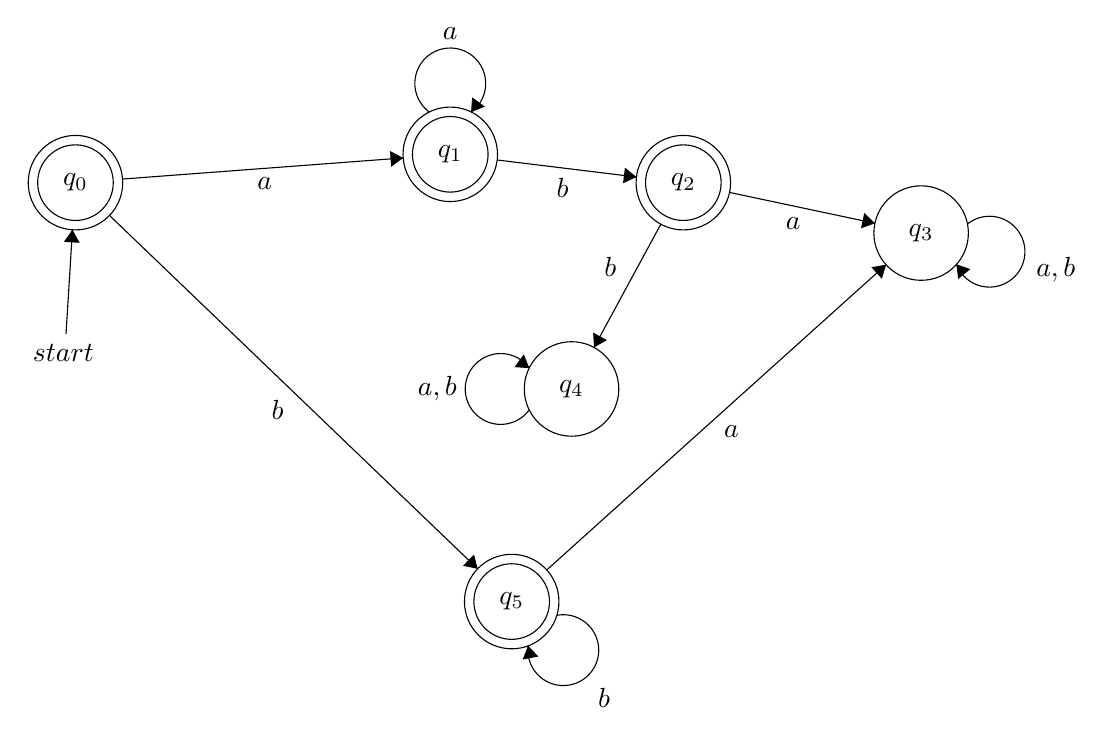
\begin{tikzpicture}[scale=0.2]
\tikzstyle{every node}+=[inner sep=0pt]
\draw [black] (12.3,-21.4) circle (3);
\draw (12.3,-21.4) node {$q_0$};
\draw [black] (12.3,-21.4) circle (2.4);
\draw [black] (36.1,-19.6) circle (3);
\draw (36.1,-19.6) node {$q_1$};
\draw [black] (36.1,-19.6) circle (2.4);
\draw [black] (50.9,-21.4) circle (3);
\draw (50.9,-21.4) node {$q_2$};
\draw [black] (50.9,-21.4) circle (2.4);
\draw [black] (66,-24.6) circle (3);
\draw (66,-24.6) node {$q_3$};
\draw [black] (43.8,-34.5) circle (3);
\draw (43.8,-34.5) node {$q_4$};
\draw [black] (40,-48) circle (3);
\draw (40,-48) node {$q_5$};
\draw [black] (40,-48) circle (2.4);
\draw [black] (15.29,-21.17) -- (33.11,-19.83);
\fill [black] (33.11,-19.83) -- (32.27,-19.39) -- (32.35,-20.39);
\draw (24.31,-21.06) node [below] {$a$};
\draw [black] (34.777,-16.92) arc (234:-54:2.25);
\draw (36.1,-12.35) node [above] {$a$};
\fill [black] (37.42,-16.92) -- (38.3,-16.57) -- (37.49,-15.98);
\draw [black] (39.08,-19.96) -- (47.92,-21.04);
\fill [black] (47.92,-21.04) -- (47.19,-20.44) -- (47.07,-21.44);
\draw (43.23,-21.09) node [below] {$b$};
\draw [black] (53.83,-22.02) -- (63.07,-23.98);
\fill [black] (63.07,-23.98) -- (62.39,-23.32) -- (62.18,-24.3);
\draw (57.88,-23.58) node [below] {$a$};
\draw [black] (68.933,-24.029) arc (128.74488:-159.25512:2.25);
\draw (73.28,-26.9) node [right] {$a,b$};
\fill [black] (68.24,-26.58) -- (68.35,-27.52) -- (69.13,-26.89);
\draw [black] (49.47,-24.04) -- (45.23,-31.86);
\fill [black] (45.23,-31.86) -- (46.05,-31.4) -- (45.17,-30.92);
\draw (46.68,-26.77) node [left] {$b$};
\draw [black] (41.12,-35.823) arc (324:36:2.25);
\draw (36.55,-34.5) node [left] {$a,b$};
\fill [black] (41.12,-33.18) -- (40.77,-32.3) -- (40.18,-33.11);
\draw [black] (42.23,-45.99) -- (63.77,-26.61);
\fill [black] (63.77,-26.61) -- (62.84,-26.77) -- (63.51,-27.51);
\draw (53.96,-36.79) node [below] {$a$};
\draw [black] (42.858,-48.874) arc (100.7357:-187.2643:2.25);
\draw (45.45,-54.09) node [right] {$b$};
\fill [black] (41.04,-50.8) -- (40.7,-51.68) -- (41.69,-51.49);
\draw [black] (14.46,-23.48) -- (37.84,-45.92);
\fill [black] (37.84,-45.92) -- (37.61,-45.01) -- (36.91,-45.73);
\draw (25.13,-35.18) node [below] {$b$};
\draw [black] (11.7,-31) -- (12.11,-24.39);
\draw (11.53,-31.63) node [below] {$start$};
\fill [black] (12.11,-24.39) -- (11.56,-25.16) -- (12.56,-25.22);
\end{tikzpicture}
\end{center}

\subsection*{b.}

\begin{center}
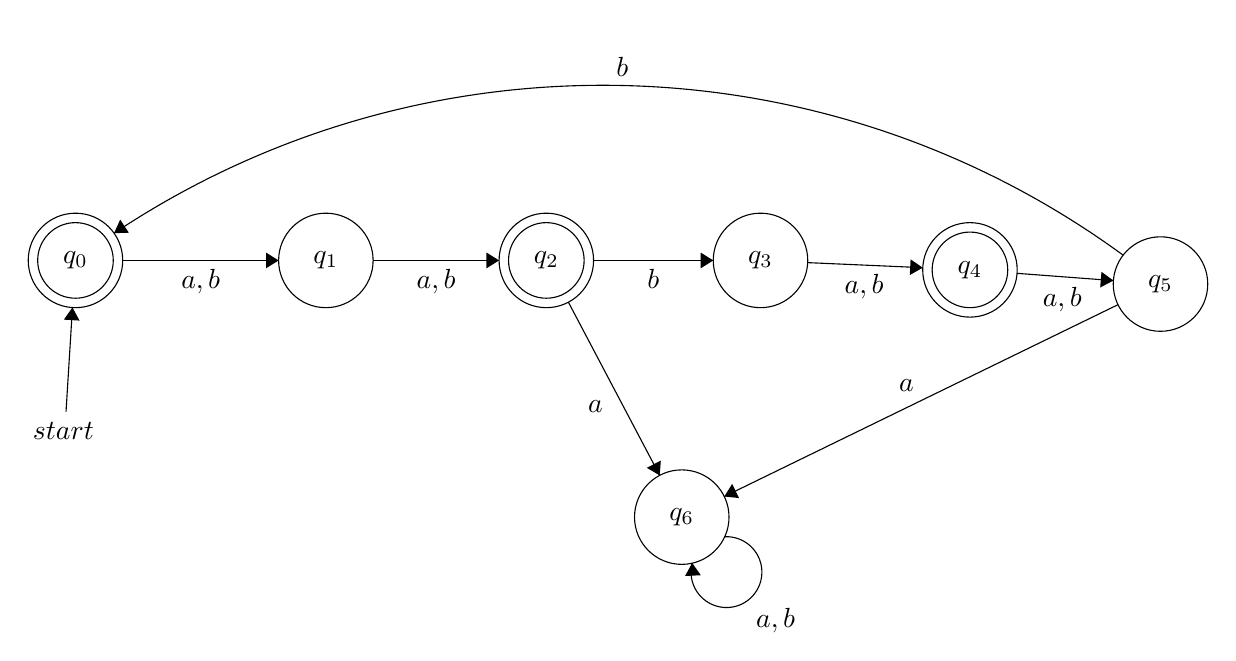
\begin{tikzpicture}[scale=0.2]
\tikzstyle{every node}+=[inner sep=0pt]
\draw [black] (4.6,-21.4) circle (3);
\draw (4.6,-21.4) node {$q_0$};
\draw [black] (4.6,-21.4) circle (2.4);
\draw [black] (20.5,-21.4) circle (3);
\draw (20.5,-21.4) node {$q_1$};
\draw [black] (34.5,-21.4) circle (3);
\draw (34.5,-21.4) node {$q_2$};
\draw [black] (34.5,-21.4) circle (2.4);
\draw [black] (48.1,-21.4) circle (3);
\draw (48.1,-21.4) node {$q_3$};
\draw [black] (61.4,-22) circle (3);
\draw (61.4,-22) node {$q_4$};
\draw [black] (61.4,-22) circle (2.4);
\draw [black] (73.5,-22.9) circle (3);
\draw (73.5,-22.9) node {$q_5$};
\draw [black] (43.1,-37.7) circle (3);
\draw (43.1,-37.7) node {$q_6$};
\draw [black] (7.6,-21.4) -- (17.5,-21.4);
\fill [black] (17.5,-21.4) -- (16.7,-20.9) -- (16.7,-21.9);
\draw (12.55,-21.9) node [below] {$a,b$};
\draw [black] (23.5,-21.4) -- (31.5,-21.4);
\fill [black] (31.5,-21.4) -- (30.7,-20.9) -- (30.7,-21.9);
\draw (27.5,-21.9) node [below] {$a,b$};
\draw [black] (37.5,-21.4) -- (45.1,-21.4);
\fill [black] (45.1,-21.4) -- (44.3,-20.9) -- (44.3,-21.9);
\draw (41.3,-21.9) node [below] {$b$};
\draw [black] (4,-31) -- (4.41,-24.39);
\draw (3.83,-31.63) node [below] {$start$};
\fill [black] (4.41,-24.39) -- (3.86,-25.16) -- (4.86,-25.22);
\draw [black] (51.1,-21.54) -- (58.4,-21.86);
\fill [black] (58.4,-21.86) -- (57.63,-21.33) -- (57.58,-22.33);
\draw (54.68,-22.27) node [below] {$a,b$};
\draw [black] (64.39,-22.22) -- (70.51,-22.68);
\fill [black] (70.51,-22.68) -- (69.75,-22.12) -- (69.67,-23.12);
\draw (67.26,-23.06) node [below] {$a,b$};
\draw [black] (70.8,-24.21) -- (45.8,-36.39);
\fill [black] (45.8,-36.39) -- (46.74,-36.49) -- (46.3,-35.59);
\draw (57.37,-29.79) node [above] {$a$};
\draw [black] (45.816,-38.946) arc (93.09386:-194.90614:2.25);
\draw (49.06,-43.43) node [below] {$a,b$};
\fill [black] (43.76,-40.61) -- (43.31,-41.44) -- (44.31,-41.39);
\draw [black] (35.9,-24.05) -- (41.7,-35.05);
\fill [black] (41.7,-35.05) -- (41.77,-34.11) -- (40.88,-34.57);
\draw (38.12,-30.71) node [left] {$a$};
\draw [black] (7.051,-19.67) arc (123.67548:53.83018:55.978);
\fill [black] (7.05,-19.67) -- (7.99,-19.64) -- (7.44,-18.81);
\draw (39.32,-9.77) node [above] {$b$};
\end{tikzpicture}
\end{center}

\subsection*{c.}

\begin{center}
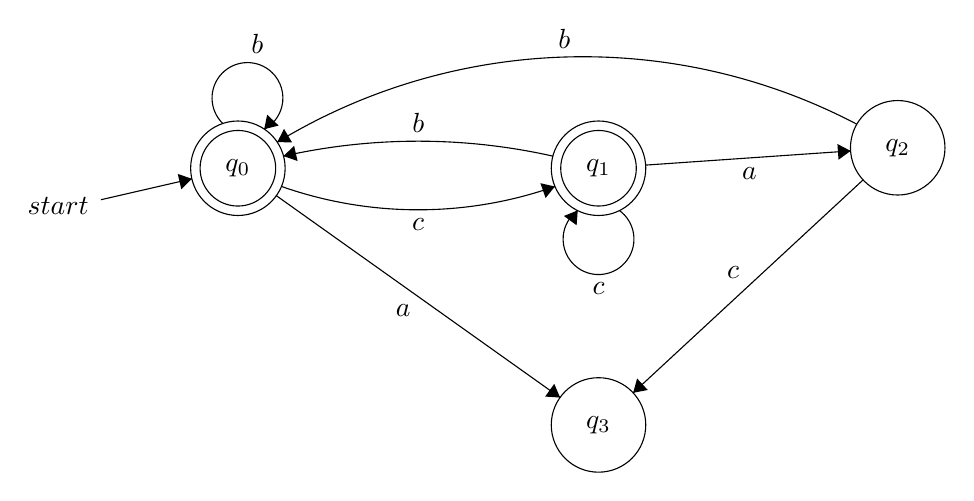
\begin{tikzpicture}[scale=0.2]
\tikzstyle{every node}+=[inner sep=0pt]
\draw [black] (16.6,-15) circle (3);
\draw (16.6,-15) node {$q_0$};
\draw [black] (16.6,-15) circle (2.4);
\draw [black] (39.5,-15) circle (3);
\draw (39.5,-15) node {$q_1$};
\draw [black] (39.5,-15) circle (2.4);
\draw [black] (58.5,-13.7) circle (3);
\draw (58.5,-13.7) node {$q_2$};
\draw [black] (39.5,-31.3) circle (3);
\draw (39.5,-31.3) node {$q_3$};
\draw [black] (7.9,-17) -- (13.68,-15.67);
\draw (7.15,-17.4) node [left] {$start$};
\fill [black] (13.68,-15.67) -- (12.78,-15.36) -- (13.01,-16.34);
\draw [black] (15.652,-12.166) arc (226.23483:-61.76517:2.25);
\draw (17.83,-7.72) node [above] {$b$};
\fill [black] (18.27,-12.52) -- (19.19,-12.29) -- (18.46,-11.6);
\draw [black] (36.733,-16.156) arc (-70.61663:-109.38337:26.163);
\fill [black] (36.73,-16.16) -- (35.81,-15.95) -- (36.14,-16.89);
\draw (28.05,-18.14) node [below] {$c$};
\draw [black] (40.823,-17.68) arc (54:-234:2.25);
\draw (39.5,-22.25) node [below] {$c$};
\fill [black] (38.18,-17.68) -- (37.3,-18.03) -- (38.11,-18.62);
\draw [black] (19.499,-14.23) arc (102.66745:77.33255:38.995);
\fill [black] (19.5,-14.23) -- (20.39,-14.54) -- (20.17,-13.57);
\draw (28.05,-12.78) node [above] {$b$};
\draw [black] (42.49,-14.8) -- (55.51,-13.9);
\fill [black] (55.51,-13.9) -- (54.67,-13.46) -- (54.74,-14.46);
\draw (49.09,-14.91) node [below] {$a$};
\draw [black] (19.1,-13.343) arc (121.23047:62.32373:37.44);
\fill [black] (19.1,-13.34) -- (20.04,-13.36) -- (19.53,-12.5);
\draw (37.33,-7.41) node [above] {$b$};
\draw [black] (56.3,-15.74) -- (41.7,-29.26);
\fill [black] (41.7,-29.26) -- (42.63,-29.08) -- (41.95,-28.35);
\draw (48.04,-22.01) node [above] {$c$};
\draw [black] (19.04,-16.74) -- (37.06,-29.56);
\fill [black] (37.06,-29.56) -- (36.69,-28.69) -- (36.11,-29.5);
\draw (27.1,-23.65) node [below] {$a$};
\end{tikzpicture}
\end{center}

\section*{Answer 3}


\subsection*{a.}

\begin{center}
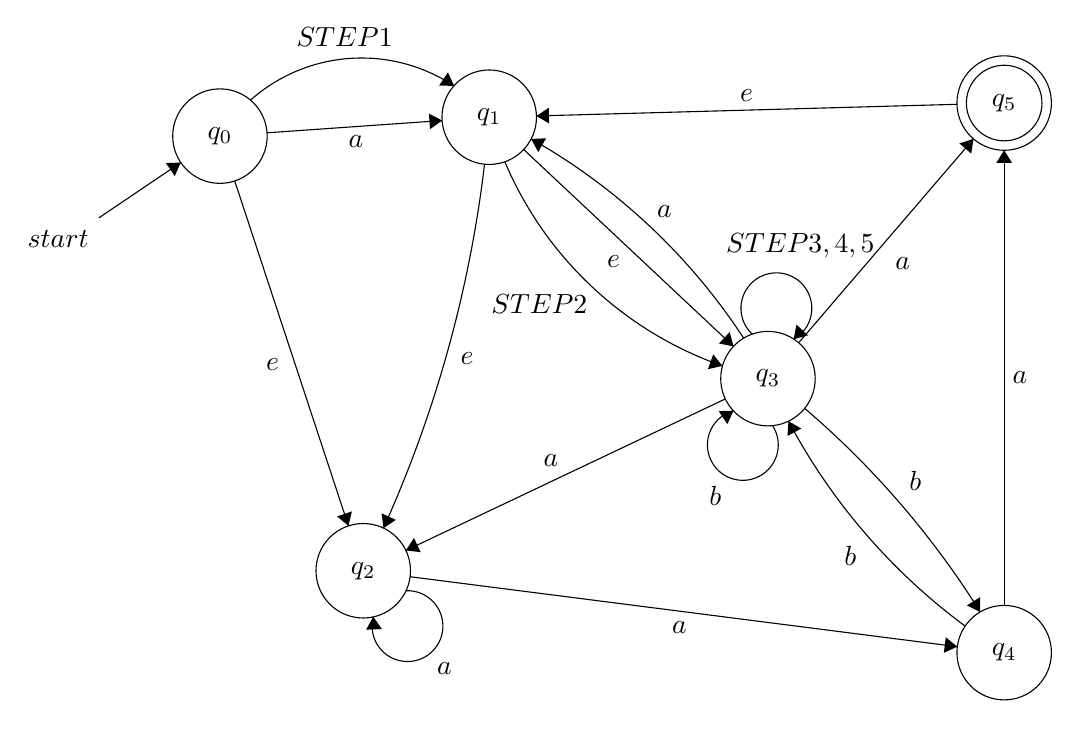
\begin{tikzpicture}[scale=0.2]
\tikzstyle{every node}+=[inner sep=0pt]
\draw [black] (13.9,-11.3) circle (3);
\draw (13.9,-11.3) node {$q_0$};
\draw [black] (31,-10.1) circle (3);
\draw (31,-10.1) node {$q_1$};
\draw [black] (23,-38.9) circle (3);
\draw (23,-38.9) node {$q_2$};
\draw [black] (48.7,-26.7) circle (3);
\draw (48.7,-26.7) node {$q_3$};
\draw [black] (63.7,-44.1) circle (3);
\draw (63.7,-44.1) node {$q_4$};
\draw [black] (63.7,-9.2) circle (3);
\draw (63.7,-9.2) node {$q_5$};
\draw [black] (63.7,-9.2) circle (2.4);
\draw [black] (6.2,-16.5) -- (11.41,-12.98);
\draw (5.59,-17.84) node [left] {$start$};
\fill [black] (11.41,-12.98) -- (10.47,-13.01) -- (11.03,-13.84);
\draw [black] (16.89,-11.09) -- (28.01,-10.31);
\fill [black] (28.01,-10.31) -- (27.17,-9.87) -- (27.24,-10.86);
\draw (22.54,-11.26) node [below] {$a$};
\draw [black] (14.84,-14.15) -- (22.06,-36.05);
\fill [black] (22.06,-36.05) -- (22.28,-35.13) -- (21.34,-35.45);
\draw (17.68,-25.79) node [left] {$e$};
\draw [black] (30.703,-13.085) arc (-6.76774:-24.28048:78.758);
\fill [black] (24.29,-36.19) -- (25.07,-35.67) -- (24.16,-35.25);
\draw (29.15,-25.42) node [right] {$e$};
\draw [black] (33.19,-12.15) -- (46.51,-24.65);
\fill [black] (46.51,-24.65) -- (46.27,-23.74) -- (45.59,-24.47);
\draw (38.89,-18.88) node [below] {$e$};
\draw [black] (25.706,-40.168) arc (92.62821:-195.37179:2.25);
\draw (28.16,-44.67) node [below] {$a$};
\fill [black] (23.64,-41.82) -- (23.18,-42.64) -- (24.18,-42.6);
\draw [black] (25.98,-39.28) -- (60.72,-43.72);
\fill [black] (60.72,-43.72) -- (59.99,-43.12) -- (59.87,-44.11);
\draw (43.08,-42.09) node [below] {$a$};
\draw [black] (33.665,-11.477) arc (60.48243:33.19126:39.199);
\fill [black] (33.66,-11.48) -- (34.11,-12.31) -- (34.61,-11.44);
\draw (42.13,-16.51) node [above] {$a$};
\draw [black] (45.99,-27.99) -- (25.71,-37.61);
\fill [black] (25.71,-37.61) -- (26.65,-37.72) -- (26.22,-36.82);
\draw (34.92,-32.29) node [above] {$a$};
\draw [black] (50.65,-24.42) -- (61.75,-11.48);
\fill [black] (61.75,-11.48) -- (60.85,-11.76) -- (61.61,-12.41);
\draw (56.75,-19.39) node [right] {$a$};
\draw [black] (48.986,-29.675) arc (33.21622:-254.78378:2.25);
\draw (45.36,-33.53) node [below] {$b$};
\fill [black] (46.51,-28.74) -- (45.57,-28.76) -- (46.12,-29.59);
\draw [black] (51.031,-28.587) arc (49.48155:32.04566:56.308);
\fill [black] (62.18,-41.52) -- (62.18,-40.57) -- (61.33,-41.1);
\draw (57.64,-33.18) node [right] {$b$};
\draw [black] (63.7,-41.1) -- (63.7,-12.2);
\fill [black] (63.7,-12.2) -- (63.2,-13) -- (64.2,-13);
\draw (64.2,-26.65) node [right] {$a$};
\draw [black] (61.221,-42.412) arc (-126.46515:-152.00764:38.855);
\fill [black] (50,-29.4) -- (49.94,-30.34) -- (50.82,-29.87);
\draw (54.34,-37.98) node [left] {$b$};
\draw [black] (60.7,-9.28) -- (34,-10.02);
\fill [black] (34,-10.02) -- (34.81,-10.5) -- (34.78,-9.5);
\draw (47.34,-9.12) node [above] {$e$};
\draw [black] (15.834,-9.02) arc (131.60184:56.42651:10.626);
\fill [black] (28.77,-8.11) -- (28.38,-7.25) -- (27.82,-8.09);
\draw (21.82,-5.65) node [above] {$STEP1$};
\draw [black] (45.813,-25.893) arc (-109.2895:-157.03681:23.411);
\fill [black] (45.81,-25.89) -- (45.22,-25.16) -- (44.89,-26.1);
\draw (34.18,-21.36) node [below] {$STEP2$};
\draw [black] (47.706,-23.882) arc (227.16338:-60.83662:2.25);
\draw (50.76,-19.07) node [above] {$STEP3,4,5$};
\fill [black] (50.33,-24.2) -- (51.24,-23.95) -- (50.51,-23.27);
\end{tikzpicture}
\end{center}

We cant reach to the end-state $q_5$ with this word so $w_1$ is not in the language.(Also there is no word that ends with b in this language since there is no empty input or b input coming in to $q_5$)

\subsection*{b.}

\begin{center}
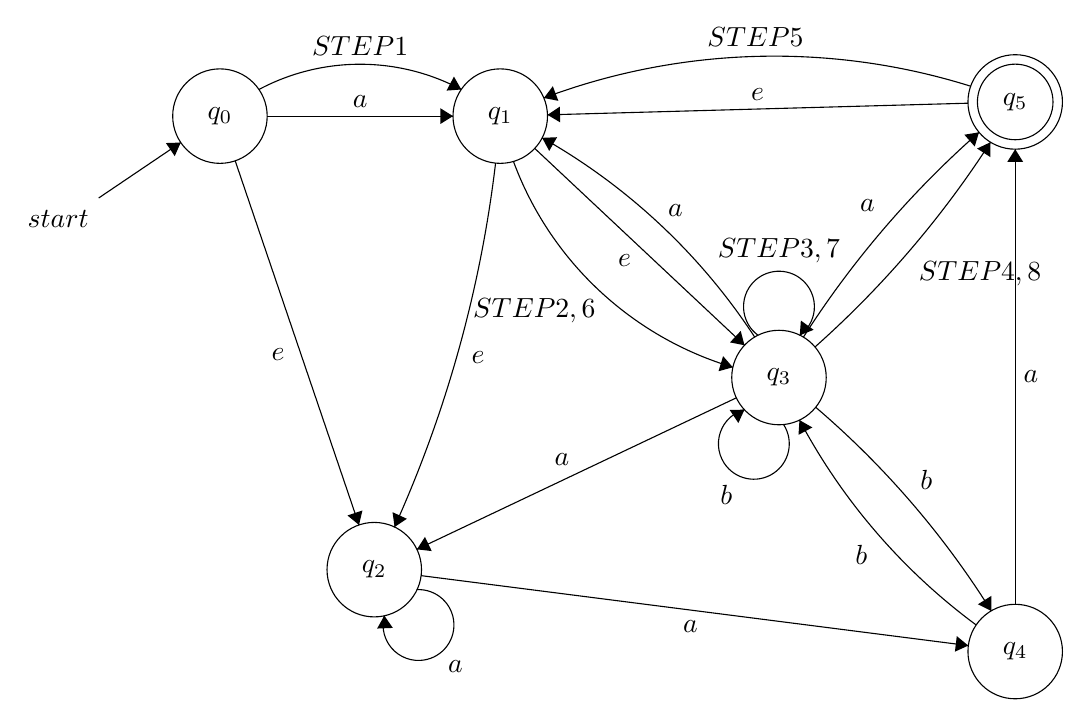
\begin{tikzpicture}[scale=0.2]
\tikzstyle{every node}+=[inner sep=0pt]
\draw [black] (13.2,-10.1) circle (3);
\draw (13.2,-10.1) node {$q_0$};
\draw [black] (31,-10.1) circle (3);
\draw (31,-10.1) node {$q_1$};
\draw [black] (23,-38.9) circle (3);
\draw (23,-38.9) node {$q_2$};
\draw [black] (48.7,-26.7) circle (3);
\draw (48.7,-26.7) node {$q_3$};
\draw [black] (63.7,-44.1) circle (3);
\draw (63.7,-44.1) node {$q_4$};
\draw [black] (63.7,-9.2) circle (3);
\draw (63.7,-9.2) node {$q_5$};
\draw [black] (63.7,-9.2) circle (2.4);
\draw [black] (5.5,-15.3) -- (10.71,-11.78);
\draw (4.89,-16.64) node [left] {$start$};
\fill [black] (10.71,-11.78) -- (9.77,-11.81) -- (10.33,-12.64);
\draw [black] (16.2,-10.1) -- (28,-10.1);
\fill [black] (28,-10.1) -- (27.2,-9.6) -- (27.2,-10.6);
\draw (22.1,-9.6) node [above] {$a$};
\draw [black] (14.17,-12.94) -- (22.03,-36.06);
\fill [black] (22.03,-36.06) -- (22.25,-35.14) -- (21.3,-35.46);
\draw (17.34,-25.22) node [left] {$e$};
\draw [black] (30.703,-13.085) arc (-6.76774:-24.28048:78.758);
\fill [black] (24.29,-36.19) -- (25.07,-35.67) -- (24.16,-35.25);
\draw (29.15,-25.42) node [right] {$e$};
\draw [black] (33.19,-12.15) -- (46.51,-24.65);
\fill [black] (46.51,-24.65) -- (46.27,-23.74) -- (45.59,-24.47);
\draw (38.89,-18.88) node [below] {$e$};
\draw [black] (25.706,-40.168) arc (92.62821:-195.37179:2.25);
\draw (28.16,-44.67) node [below] {$a$};
\fill [black] (23.64,-41.82) -- (23.18,-42.64) -- (24.18,-42.6);
\draw [black] (25.98,-39.28) -- (60.72,-43.72);
\fill [black] (60.72,-43.72) -- (59.99,-43.12) -- (59.87,-44.11);
\draw (43.08,-42.09) node [below] {$a$};
\draw [black] (33.665,-11.477) arc (60.48243:33.19126:39.199);
\fill [black] (33.66,-11.48) -- (34.11,-12.31) -- (34.61,-11.44);
\draw (42.13,-16.51) node [above] {$a$};
\draw [black] (45.99,-27.99) -- (25.71,-37.61);
\fill [black] (25.71,-37.61) -- (26.65,-37.72) -- (26.22,-36.82);
\draw (34.92,-32.29) node [above] {$a$};
\draw [black] (50.253,-24.133) arc (147.4266:131.37081:61.331);
\fill [black] (61.4,-11.13) -- (60.47,-11.28) -- (61.13,-12.03);
\draw (54.82,-15.79) node [left] {$a$};
\draw [black] (48.986,-29.675) arc (33.21622:-254.78378:2.25);
\draw (45.36,-33.53) node [below] {$b$};
\fill [black] (46.51,-28.74) -- (45.57,-28.76) -- (46.12,-29.59);
\draw [black] (51.031,-28.587) arc (49.48155:32.04566:56.308);
\fill [black] (62.18,-41.52) -- (62.18,-40.57) -- (61.33,-41.1);
\draw (57.64,-33.18) node [right] {$b$};
\draw [black] (63.7,-41.1) -- (63.7,-12.2);
\fill [black] (63.7,-12.2) -- (63.2,-13) -- (64.2,-13);
\draw (64.2,-26.65) node [right] {$a$};
\draw [black] (61.221,-42.412) arc (-126.46515:-152.00764:38.855);
\fill [black] (50,-29.4) -- (49.94,-30.34) -- (50.82,-29.87);
\draw (54.34,-37.98) node [left] {$b$};
\draw [black] (60.7,-9.28) -- (34,-10.02);
\fill [black] (34,-10.02) -- (34.81,-10.5) -- (34.78,-9.5);
\draw (47.34,-9.12) node [above] {$e$};
\draw [black] (15.672,-8.411) arc (118.05427:61.94573:13.667);
\fill [black] (28.53,-8.41) -- (28.06,-7.59) -- (27.59,-8.48);
\draw (22.1,-6.31) node [above] {$STEP1$};
\draw [black] (45.774,-26.047) arc (-106.60574:-159.72057:21.366);
\fill [black] (45.77,-26.05) -- (45.15,-25.34) -- (44.86,-26.3);
\draw (33.16,-21.64) node [below] {$STEP2,6$};
\draw [black] (47.377,-24.02) arc (234:-54:2.25);
\draw (48.7,-19.45) node [above] {$STEP3,7$};
\fill [black] (50.02,-24.02) -- (50.9,-23.67) -- (50.09,-23.08);
\draw [black] (62.133,-11.758) arc (-32.83757:-48.36502:63.385);
\fill [black] (62.13,-11.76) -- (61.28,-12.16) -- (62.12,-12.7);
\draw (57.55,-20.08) node [right] {$STEP4,8$};
\draw [black] (33.769,-8.946) arc (110.56113:72.59197:41.673);
\fill [black] (33.77,-8.95) -- (34.69,-9.13) -- (34.34,-8.2);
\draw (47.21,-5.72) node [above] {$STEP5$};
\end{tikzpicture}
\end{center}

We can reach to the end-state $q_5$ by following the path $q_0 \implies q_1 \implies q_3 \implies q_3 \implies q_5 \implies q_1 \implies q_3 \implies q_3 \implies q_5$. 
\\
So we can read the word $ababa$ in this language, therefore this word is in the language.


\section*{Answer 4}

\subsection*{a.}

A generalized finite autoamaton (GFA) has one starting state with no incoming transitions; one final state with no outgoing transitions.
\\
Therefore our GFA is of the form:

\begin{center}
\begin{tikzpicture}[scale=0.2]
\tikzstyle{every node}+=[inner sep=0pt]
\draw [black] (11.1,-8.4) circle (3);
\draw (11.1,-8.4) node {$q_4$};
\draw [black] (25.6,-12.7) circle (3);
\draw (25.6,-12.7) node {$q_0$};
\draw [black] (38.7,-12.7) circle (3);
\draw (38.7,-12.7) node {$q_1$};
\draw [black] (56,-13.2) circle (3);
\draw (56,-13.2) node {$q_2$};
\draw [black] (73.7,-24.6) circle (3);
\draw (73.7,-24.6) node {$q_5$};
\draw [black] (73.7,-24.6) circle (2.4);
\draw [black] (43.4,-29.5) circle (3);
\draw (43.4,-29.5) node {$q_3$};
\draw [black] (5,-3.6) -- (8.74,-6.54);
\draw (4.43,-2.18) node [left] {$start$};
\fill [black] (8.74,-6.54) -- (8.42,-5.66) -- (7.8,-6.44);
\draw [black] (13.98,-9.25) -- (22.72,-11.85);
\fill [black] (22.72,-11.85) -- (22.1,-11.14) -- (21.81,-12.1);
\draw (17.57,-11.1) node [below] {$e$};
\draw [black] (28.6,-12.7) -- (35.7,-12.7);
\fill [black] (35.7,-12.7) -- (34.9,-12.2) -- (34.9,-13.2);
\draw (32.15,-13.2) node [below] {$b$};
\draw [black] (41.64,-12.108) arc (98.69514:77.99388:31.903);
\fill [black] (53.1,-12.44) -- (52.42,-11.78) -- (52.21,-12.76);
\draw (47.4,-11.23) node [above] {$a$};
\draw [black] (53.137,-14.09) arc (-76.5703:-106.74067:22.355);
\fill [black] (41.51,-13.75) -- (42.13,-14.46) -- (42.42,-13.51);
\draw (47.28,-15.22) node [below] {$b$};
\draw [black] (58.616,-14.645) arc (88.82449:-199.17551:2.25);
\draw (60.86,-19.24) node [below] {$b$};
\fill [black] (56.44,-16.16) -- (55.93,-16.94) -- (56.93,-16.97);
\draw [black] (54.17,-15.57) -- (45.23,-27.13);
\fill [black] (45.23,-27.13) -- (46.12,-26.8) -- (45.33,-26.19);
\draw (49.13,-19.94) node [left] {$b$};
\draw [black] (46.23,-30.46) arc (99:-189:2.25);
\draw (48.7,-35.75) node [right] {$a$};
\fill [black] (44.36,-32.33) -- (43.99,-33.2) -- (44.98,-33.04);
\draw [black] (40.297,-15.238) arc (28.82287:2.43632:25.624);
\fill [black] (43.45,-26.5) -- (43.91,-25.68) -- (42.91,-25.72);
\draw (43.29,-20.14) node [right] {$e$};
\draw [black] (41.084,-27.604) arc (-135.85346:-192.88735:13.138);
\fill [black] (37.7,-15.52) -- (37.04,-16.19) -- (38.01,-16.41);
\draw (37.09,-22.54) node [left] {$b$};
\draw [black] (28,-10.903) arc (123.07777:55.03767:22.936);
\fill [black] (28,-10.9) -- (28.94,-10.89) -- (28.4,-10.05);
\draw (40.9,-6.67) node [above] {$a$};
\draw [black] (58.929,-13.842) arc (74.35849:40.07295:26.181);
\fill [black] (71.9,-22.2) -- (71.77,-21.26) -- (71.01,-21.91);
\draw (66.99,-16.54) node [above] {$e$};
\draw [black] (46.36,-29.02) -- (70.74,-25.08);
\fill [black] (70.74,-25.08) -- (69.87,-24.71) -- (70.03,-25.7);
\draw (58.94,-27.64) node [below] {$e$};
\end{tikzpicture}
\end{center}


\subsection*{b.}

Continuing from the first state given in 4.a:
\\
\\
Eleminate $q_0$ :
\\
\begin{center}
\begin{tikzpicture}[scale=0.2]
\tikzstyle{every node}+=[inner sep=0pt]
\draw [black] (11.1,-8.4) circle (3);
\draw (11.1,-8.4) node {$q_4$};
\draw [black] (38.7,-12.7) circle (3);
\draw (38.7,-12.7) node {$q_1$};
\draw [black] (56.1,-12.7) circle (3);
\draw (56.1,-12.7) node {$q_2$};
\draw [black] (73.7,-24.6) circle (3);
\draw (73.7,-24.6) node {$q_5$};
\draw [black] (73.7,-24.6) circle (2.4);
\draw [black] (43.4,-29.5) circle (3);
\draw (43.4,-29.5) node {$q_3$};
\draw [black] (5,-3.6) -- (8.74,-6.54);
\draw (4.43,-2.18) node [left] {$start$};
\fill [black] (8.74,-6.54) -- (8.42,-5.66) -- (7.8,-6.44);
\draw [black] (41.7,-12.7) -- (53.1,-12.7);
\fill [black] (53.1,-12.7) -- (52.3,-12.2) -- (52.3,-13.2);
\draw (47.4,-13.2) node [below] {$a$};
\draw [black] (40.051,-10.037) arc (143.67303:36.32697:9.121);
\fill [black] (40.05,-10.04) -- (40.93,-9.69) -- (40.12,-9.1);
\draw (47.4,-5.82) node [above] {$ab\mbox{ }U\mbox{ }b$};
\draw [black] (58.716,-14.145) arc (88.82449:-199.17551:2.25);
\draw (60.96,-18.74) node [below] {$b$};
\fill [black] (56.54,-15.66) -- (56.03,-16.44) -- (57.03,-16.47);
\draw [black] (54.29,-15.09) -- (45.21,-27.11);
\fill [black] (45.21,-27.11) -- (46.09,-26.77) -- (45.29,-26.17);
\draw (49.17,-19.7) node [left] {$b$};
\draw [black] (46.23,-30.46) arc (99:-189:2.25);
\draw (48.7,-35.75) node [right] {$a$};
\fill [black] (44.36,-32.33) -- (43.99,-33.2) -- (44.98,-33.04);
\draw [black] (40.297,-15.238) arc (28.82287:2.43632:25.624);
\fill [black] (43.45,-26.5) -- (43.91,-25.68) -- (42.91,-25.72);
\draw (43.29,-20.14) node [right] {$e$};
\draw [black] (41.084,-27.604) arc (-135.85346:-192.88735:13.138);
\fill [black] (37.7,-15.52) -- (37.04,-16.19) -- (38.01,-16.41);
\draw (37.09,-22.54) node [left] {$b$};
\draw [black] (59.012,-13.415) arc (72.98414:38.88775:26.64);
\fill [black] (71.95,-22.16) -- (71.84,-21.23) -- (71.06,-21.86);
\draw (67.08,-16.32) node [above] {$e$};
\draw [black] (46.36,-29.02) -- (70.74,-25.08);
\fill [black] (70.74,-25.08) -- (69.87,-24.71) -- (70.03,-25.7);
\draw (58.94,-27.64) node [below] {$e$};
\draw [black] (14.06,-8.86) -- (35.74,-12.24);
\fill [black] (35.74,-12.24) -- (35.02,-11.62) -- (34.87,-12.61);
\draw (24.5,-11.14) node [below] {$b$};
\end{tikzpicture}
\end{center}


Eleminate $q_2$:
\\
\begin{center}
\begin{tikzpicture}[scale=0.2]
\tikzstyle{every node}+=[inner sep=0pt]
\draw [black] (11.1,-8.4) circle (3);
\draw (11.1,-8.4) node {$q_4$};
\draw [black] (29.9,-13) circle (3);
\draw (29.9,-13) node {$q_1$};
\draw [black] (73.7,-24.6) circle (3);
\draw (73.7,-24.6) node {$q_5$};
\draw [black] (73.7,-24.6) circle (2.4);
\draw [black] (38.3,-32.5) circle (3);
\draw (38.3,-32.5) node {$q_3$};
\draw [black] (5,-3.6) -- (8.74,-6.54);
\draw (4.43,-2.18) node [left] {$start$};
\fill [black] (8.74,-6.54) -- (8.42,-5.66) -- (7.8,-6.44);
\draw [black] (41.13,-33.46) arc (99:-189:2.25);
\draw (43.6,-38.75) node [right] {$a$};
\fill [black] (39.26,-35.33) -- (38.89,-36.2) -- (39.88,-36.04);
\draw [black] (31.723,-15.382) arc (35.1433:11.46648:37.57);
\fill [black] (37.82,-29.54) -- (38.15,-28.66) -- (37.17,-28.85);
\draw (36.24,-21.18) node [right] {$e\mbox{ }U\mbox{ }ab^*b$};
\draw [black] (35.892,-30.717) arc (-131.14026:-182.24996:18.604);
\fill [black] (29.54,-15.98) -- (29.01,-16.75) -- (30.01,-16.79);
\draw (30.31,-25.03) node [left] {$b$};
\draw [black] (41.23,-31.85) -- (70.77,-25.25);
\fill [black] (70.77,-25.25) -- (69.88,-24.94) -- (70.1,-25.92);
\draw (56.6,-29.13) node [below] {$e$};
\draw [black] (14.01,-9.11) -- (26.99,-12.29);
\fill [black] (26.99,-12.29) -- (26.33,-11.61) -- (26.09,-12.58);
\draw (19.79,-11.27) node [below] {$b$};
\draw [black] (30.081,-10.017) arc (204.25512:-83.74488:2.25);
\draw (39.67,-6.63) node [above] {$(ab^*(ab\mbox{ }U\mbox{ }b))^*$};
\fill [black] (32.38,-11.33) -- (33.31,-11.46) -- (32.9,-10.55);
\draw [black] (32.8,-13.77) -- (70.8,-23.83);
\fill [black] (70.8,-23.83) -- (70.15,-23.14) -- (69.9,-24.11);
\draw (53.61,-18.15) node [above] {$ab^*e$};
\end{tikzpicture}
\end{center}


Eleminate $q_3$ :
\\
\begin{center}
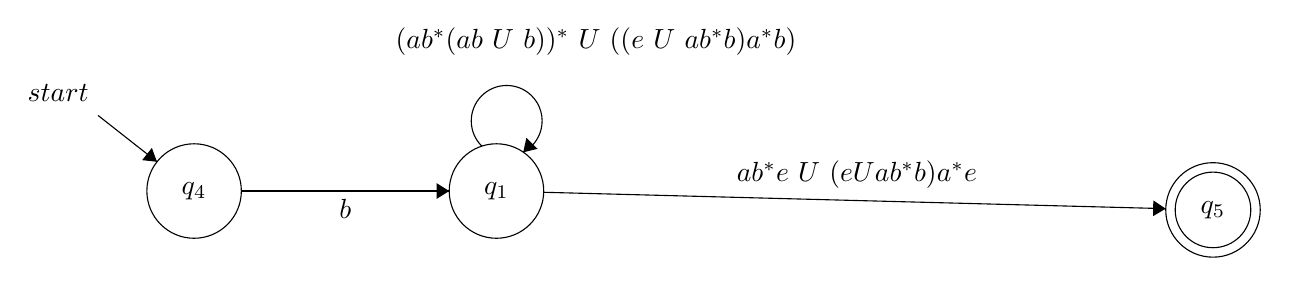
\begin{tikzpicture}[scale=0.2]
\tikzstyle{every node}+=[inner sep=0pt]
\draw [black] (10.7,-11.8) circle (3);
\draw (10.7,-11.8) node {$q_4$};
\draw [black] (29.9,-11.8) circle (3);
\draw (29.9,-11.8) node {$q_1$};
\draw [black] (75.4,-13) circle (3);
\draw (75.4,-13) node {$q_5$};
\draw [black] (75.4,-13) circle (2.4);
\draw [black] (4.6,-7) -- (8.34,-9.94);
\draw (4.03,-5.58) node [left] {$start$};
\fill [black] (8.34,-9.94) -- (8.02,-9.06) -- (7.4,-9.84);
\draw [black] (13.7,-11.8) -- (26.9,-11.8);
\fill [black] (26.9,-11.8) -- (26.1,-11.3) -- (26.1,-12.3);
\draw (20.3,-12.3) node [below] {$b$};
\draw [black] (28.978,-8.958) arc (225.70561:-62.29439:2.25);
\draw (36.22,-3.22) node [above] {$(ab^*(ab\mbox{ }U\mbox{ }b))^*\mbox{ }U\mbox{ }((e\mbox{ }U\mbox{ }ab^*b)a^*b)$};
\fill [black] (31.6,-9.34) -- (32.51,-9.12) -- (31.8,-8.42);
\draw [black] (32.9,-11.88) -- (72.4,-12.92);
\fill [black] (72.4,-12.92) -- (71.61,-12.4) -- (71.59,-13.4);
\draw (52.79,-11.65) node [above] {$ab^*e\mbox{ }U\mbox{ }(eUab^*b)a^*e$};
\end{tikzpicture}
\end{center}


Eleminate $q_1$ and simplify:
\\
\begin{center}
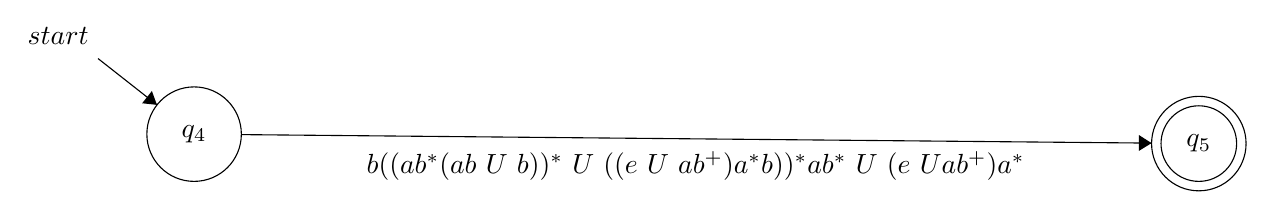
\begin{tikzpicture}[scale=0.2]
\tikzstyle{every node}+=[inner sep=0pt]
\draw [black] (10.7,-11.8) circle (3);
\draw (10.7,-11.8) node {$q_4$};
\draw [black] (74.5,-12.4) circle (3);
\draw (74.5,-12.4) node {$q_5$};
\draw [black] (74.5,-12.4) circle (2.4);
\draw [black] (4.6,-7) -- (8.34,-9.94);
\draw (4.03,-5.58) node [left] {$start$};
\fill [black] (8.34,-9.94) -- (8.02,-9.06) -- (7.4,-9.84);
\draw [black] (13.7,-11.83) -- (71.5,-12.37);
\fill [black] (71.5,-12.37) -- (70.7,-11.86) -- (70.7,-12.86);
\draw (42.55,-12.85) node [below] {$b((ab^*(ab\mbox{ }U\mbox{ }b))^*\mbox{ }U\mbox{ }((e\mbox{ }U\mbox{ }ab^+)a^*b))^*ab^*\mbox{ }U\mbox{ }(e\mbox{ }Uab^+)a^*$};
\end{tikzpicture}
\end{center}



\section*{Answer 5}

$N= \{ k,\sum,\Delta,s,F \}$
\\
$M= \{ k',\sum,\Delta,s',F' \}$

\subsection*{a.}
The algorithm is like this:
1- Create a start state of the DFA by taking E(q): (the set of states of N that can be reached from q wihtout reading any symbol from the input tape) with parameter $q_0$(stand state).
\\
So $s' = E(q_0)=\{ q_0,q_1,q_2  \}$
\\
2- Each time a new state is generated repeat these:
\\
 2.1- Create new states reachable frın tge new states by reading one symbol.
\\
2.2- Apply E() to the new states, possibly resulting in a new state.
\\
3- Finish states of M are those which contain any of the finish states of N(i.e any state that contains $q_3$)
\\
Applying second step we get:
\\
$E(q_0) = \{ q_0, q_1, q_2\}= s'$
\\
$E(q_1) = \{ q_1 \}$
\\
$E(q_2) = \{ q_2 \}$
\\
$E(q_3) = \{ q_1, q_3 \}$
\\
$\delta (E(q_0),a) = E(q_1) U E(q_3)= \{ q_1,q_3\} $
\\
$\delta (E(q_0),b) = E(q_2)= \{ q_2 \} $
\\
$\delta (E(q_1),a) =  \{ \} $
\\
$\delta (E(q_1),b) =  \{ \} $
\\
$\delta (E(q_2),a) = E(q_3)= \{ q_1,q_3\} $
\\
$\delta (E(q_2),b) = \{ \} $
\\
$\delta (E(q_3),a) = \{ \} $
\\
$\delta (E(q_3),b) = E(q_1)= \{ q_1\} $
\\
So M=
\\
\begin{center}
\begin{tikzpicture}[scale=0.2]
\tikzstyle{every node}+=[inner sep=0pt]
\draw [black] (16.7,-11.4) circle (3);
\draw (16.7,-11.4) node {$q_0,q_1,q_2$};
\draw [black] (48.7,-10.9) circle (3);
\draw (48.7,-10.9) node {$q_1,q_3$};
\draw [black] (48.7,-10.9) circle (2.4);
\draw [black] (38.8,-25.3) circle (3);
\draw (38.8,-25.3) node {$q_2$};
\draw [black] (66.5,-10.9) circle (3);
\draw (66.5,-10.9) node {$q_1$};
\draw [black] (61.1,-34.9) circle (3);
\draw (61.1,-34.9) node {$\mbox{ }\{ \} $};
\draw [black] (9.6,-14.9) -- (14.01,-12.73);
\draw (8.9,-15.99) node [left] {$start$};
\fill [black] (14.01,-12.73) -- (13.07,-12.63) -- (13.51,-13.53);
\draw [black] (19.7,-11.35) -- (45.7,-10.95);
\fill [black] (45.7,-10.95) -- (44.89,-10.46) -- (44.91,-11.46);
\draw (32.7,-11.66) node [below] {$a$};
\draw [black] (19.24,-13) -- (36.26,-23.7);
\fill [black] (36.26,-23.7) -- (35.85,-22.85) -- (35.32,-23.7);
\draw (26.75,-18.85) node [below] {$b$};
\draw [black] (40.5,-22.83) -- (47,-13.37);
\fill [black] (47,-13.37) -- (46.14,-13.75) -- (46.96,-14.31);
\draw (44.35,-19.45) node [right] {$a$};
\draw [black] (41.56,-26.49) -- (58.34,-33.71);
\fill [black] (58.34,-33.71) -- (57.81,-32.94) -- (57.41,-33.86);
\draw (48.98,-30.61) node [below] {$b$};
\draw [black] (50.08,-13.57) -- (59.72,-32.23);
\fill [black] (59.72,-32.23) -- (59.8,-31.29) -- (58.91,-31.75);
\draw (54.21,-24.04) node [left] {$a$};
\draw [black] (63.343,-36.874) arc (76.38014:-211.61986:2.25);
\draw (65.3,-41.67) node [below] {$a,b$};
\fill [black] (60.9,-37.88) -- (60.22,-38.54) -- (61.19,-38.78);
\draw [black] (65.84,-13.83) -- (61.76,-31.97);
\fill [black] (61.76,-31.97) -- (62.42,-31.3) -- (61.45,-31.08);
\draw (63.05,-22.52) node [left] {$a,b$};
\draw [black] (51.7,-10.9) -- (63.5,-10.9);
\fill [black] (63.5,-10.9) -- (62.7,-10.4) -- (62.7,-11.4);
\draw (57.6,-11.4) node [below] {$b$};
\end{tikzpicture}
\end{center}

\subsection*{b.}

We can get the complement of a DFA just by swapping end-states and non-end-states. 
\\
Since N=M, L=L(N)=L(M)
\\
If we take the complement of L we get :
\\
\begin{center}
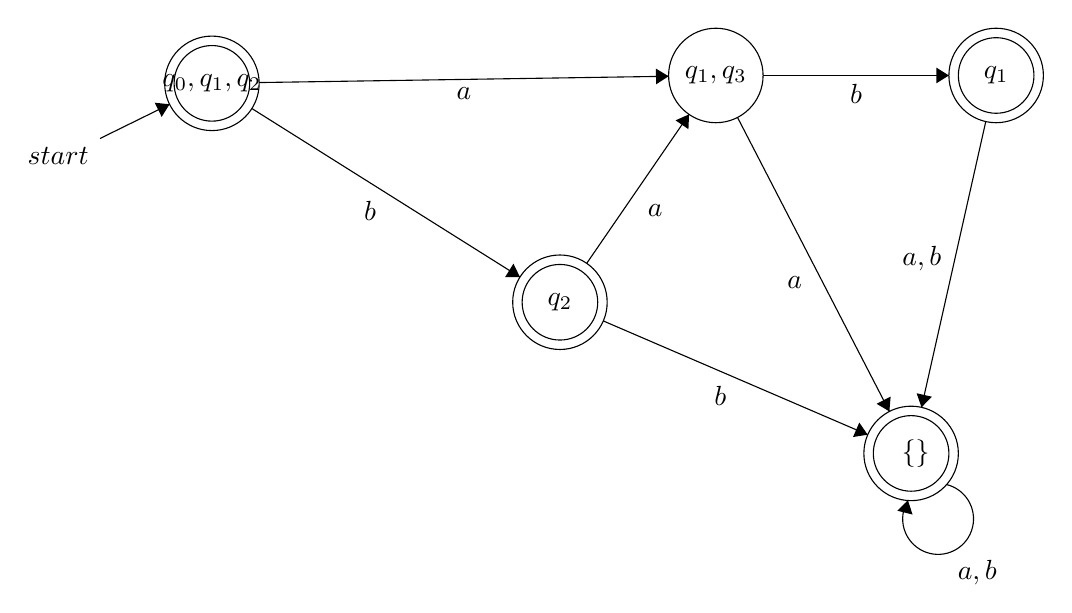
\begin{tikzpicture}[scale=0.2]
\tikzstyle{every node}+=[inner sep=0pt]
\draw [black] (16.7,-11.4) circle (3);
\draw (16.7,-11.4) node {$q_0,q_1,q_2$};
\draw [black] (16.7,-11.4) circle (2.4);
\draw [black] (48.7,-10.9) circle (3);
\draw (48.7,-10.9) node {$q_1,q_3$};
\draw [black] (38.8,-25.3) circle (3);
\draw (38.8,-25.3) node {$q_2$};
\draw [black] (38.8,-25.3) circle (2.4);
\draw [black] (66.5,-10.9) circle (3);
\draw (66.5,-10.9) node {$q_1$};
\draw [black] (66.5,-10.9) circle (2.4);
\draw [black] (61.1,-34.9) circle (3);
\draw (61.1,-34.9) node {$\mbox{ }\{ \}$};
\draw [black] (61.1,-34.9) circle (2.4);
\draw [black] (9.6,-14.9) -- (14.01,-12.73);
\draw (8.9,-15.99) node [left] {$start$};
\fill [black] (14.01,-12.73) -- (13.07,-12.63) -- (13.51,-13.53);
\draw [black] (19.7,-11.35) -- (45.7,-10.95);
\fill [black] (45.7,-10.95) -- (44.89,-10.46) -- (44.91,-11.46);
\draw (32.7,-11.66) node [below] {$a$};
\draw [black] (19.24,-13) -- (36.26,-23.7);
\fill [black] (36.26,-23.7) -- (35.85,-22.85) -- (35.32,-23.7);
\draw (26.75,-18.85) node [below] {$b$};
\draw [black] (40.5,-22.83) -- (47,-13.37);
\fill [black] (47,-13.37) -- (46.14,-13.75) -- (46.96,-14.31);
\draw (44.35,-19.45) node [right] {$a$};
\draw [black] (41.56,-26.49) -- (58.34,-33.71);
\fill [black] (58.34,-33.71) -- (57.81,-32.94) -- (57.41,-33.86);
\draw (48.98,-30.61) node [below] {$b$};
\draw [black] (50.08,-13.57) -- (59.72,-32.23);
\fill [black] (59.72,-32.23) -- (59.8,-31.29) -- (58.91,-31.75);
\draw (54.21,-24.04) node [left] {$a$};
\draw [black] (63.343,-36.874) arc (76.38014:-211.61986:2.25);
\draw (65.3,-41.67) node [below] {$a,b$};
\fill [black] (60.9,-37.88) -- (60.22,-38.54) -- (61.19,-38.78);
\draw [black] (65.84,-13.83) -- (61.76,-31.97);
\fill [black] (61.76,-31.97) -- (62.42,-31.3) -- (61.45,-31.08);
\draw (63.05,-22.52) node [left] {$a,b$};
\draw [black] (51.7,-10.9) -- (63.5,-10.9);
\fill [black] (63.5,-10.9) -- (62.7,-10.4) -- (62.7,-11.4);
\draw (57.6,-11.4) node [below] {$b$};
\end{tikzpicture}
\end{center}

Which is $e U (ba U a)((ba U bb)(a U b)^*) U (ba U a)a(a U b)^*) U b U bb(a U b)^*$ as a RE.
\\
So $\bar{L}=\sum^* - L$ or $\bar{L} = \{ w | w \in \sum^* \land w \not \in  L\} $


\section*{Answer 6}

$L_1 -  L_2 = L_1 \cap \bar{L_2}$
\\
Let $L_1= \{ Q_1, \sum, \delta_1, q_1,F_1 \}$
\\
$L_2=\{  Q_2,\sum, \delta_2, q_2, F_2 \}$
\\
so $\bar{L_2}=\{  Q_2,\sum, \delta_2, q_2,Q_2-  F_2 \}$(From Question 5.b)
\\
\\
We can assume that alphabets of the $L_1 \ and \ \bar{L_2}$ are the same i.e $\sum$ is the union of the alphabets of $L_1$ and $L_2$.
\\
We can assume that both automata are deterministic since we can convert NFA to DFA(from question 5.a)
\\
Now we should construct an automata L=$ L_1 \cap \bar{L_2}$ that simulates both $L_1 \ and \ \bar{L_2}$.
\\
States of L are pairs of states (p,q) p coming from $L_1$, q coming from $\bar{L_2}$.
\\
If p goes to s upon reading input s and q goes to t upon reading input s then in our automata L (p,q) will go to (s,t) upon reading input s.
\\
Our start state is pair of start states ($q_1,q_2$).
\\
Our end-states are pairs that are end-states in their respective automatas i.e (p,q) s.t $p \in F_1, q\in (Q_2 - F_2)$ 
\\
So our new automata $L=(Q_1 \times Q_2, \sum, \delta, (q_1,q_2), F_1 \times (Q_2 - F_2))$ where $\delta((p,q),a)= (\delta_1(p,q),\delta_2(q,a))$


\section*{Answer 7}

\subsection*{a.}

Assume L is regular
\\
If it is regular there exists some number p which is the pumping length.
\\
$w=a^{p^2}b^* \in L \ \ \ \ \mid w\mid \geq p^2 > p$ 
\\
Partition w into xyz i.e w=xyz with $\mid xy \mid \leq p$ and y shouldn't be empty.
\\
For each different way of partitioning we should show that $xy^iz \not \in L$ for some $i \geq 0$
\\
$\mid xy \mid \leq p^2 $ and y is nonempty
\\
choose $x=a^l \ \ \ y=a^m \ \ \ t= a^{p^2-l-m}$ where $l+m \leq p \ \ \ and\  m > 0$
\\
choose i=2. We get $xy^2z=a^{p^2+m} $
\\ 
$ p^2+m$ is not a perfect square since $0 > m \leq p$ and difference between $p^2$ adn next square is always greater than p for all natural numbers. 
\\
$xy^2z \not \in L$ so our assumption is wrong and L is not regular.






\end{document}

​

